\documentclass[12pt]{article}\usepackage[margin=1in]{geometry}\usepackage{amsmath,amssymb,amsthm,booktabs,graphicx,natbib,microtype}\newtheorem{theorem}{Theorem}\newtheorem{remark}[theorem]{Remark}
\title{Ten Layers of Gauge and Recurrence\\\large Closed Algebra, Finite Barriers, and the Refined Physical Frontier}\author{Prime Dynamics Theory Program}\date{July 2026}
\begin{document}\maketitle
\begin{abstract}
We audit RH-120--RH-129 as one proof system.  Five layers are constructive,
two establish obstructions, and three synthesize the route.  Gauge-covariant
Rayleigh transfer, optimal exact-Gram alignment, additive defect recurrence,
normalization exponents, combined directional support, outward validation,
and conditional eventual support are now exact.  Two shortcuts are sharply
blocked: forced common coordinates and unguarded independent assembly.
Finite evidence separates the remaining mechanisms: all 24 regularized
directional chains survive above $10^{-8}$, whereas all 24 scalar direct
margin chains lose positivity.  Neither observation is asymptotic.  The
inclusion-minimal mathematical frontier is
\[
\{P_D\},\qquad\{P_T\},\qquad\{P_R,P_A\},
\]
where $P_D$ is a physical direct recurrence, $P_T$ a physical
trace--concentration packet, $P_R$ an all-level subunit Rayleigh recurrence,
and $P_A$ a positive normalized-base liminf.  Independently assembled
validation also requires all-level outward radii.  None of these physical
packets is proved.
\end{abstract}
\section{Layer ledger}
\begin{table}[h]\centering\small
\begin{tabular}{rlll}\toprule
layer&class&principal result&route effect\\\midrule
120&constructive&gauge gamma/volume transfer&cross-level algebra opened\\
121&constructive&optimal exact-Gram gauge&intrinsic tail inflation exposed\\
122&negative&fixed-coordinate blow-up&no-gauge shortcut closed\\
123&constructive&affine defect recurrence&outward errors admitted\\
124&constructive&normalization exponents&separate-factor loss quantified\\
125&synthesis&combined directional transfer&regularized finite chains joined\\
126&negative&direct scalar-profile barrier&simple fallback held\\
127&constructive&outward Loewner guards&independent validation logic closed\\
128&synthesis&conditional liminf floor&directional algebra conditionally closed\\
129&synthesis&proof-frontier review&roadmap revised\\\bottomrule
\end{tabular}\caption{Primary classification of the ten layers.}\end{table}

All nine upstream summaries pass machine-checked curated claims.  In
particular, RH-121 has 96 optimal-gauge pairs and 25 contractive tail
factors; RH-125 has 24 regularized chains above $10^{-8}$; RH-126 has zero
positive terminal direct chains; and RH-127 validates 4,096 random outward
enclosures with zero false certifications.

\section{What is now exact}
The directional chain can be written without hidden algebra.  RH-123 gives
\[
x_{n+1}=\gamma_{n+1}^2\leq\rho_nx_n+q_n.
\]
RH-125 transports the determinant, leading scale, and capacity on the same
gauge.  RH-127 specifies the exact spectral-radius subtraction needed when
the matrices come from independent assemblies.  RH-128 then proves that
eventual caps $\rho_n\leq\rho<1$, $q_n\leq q$, with
$q/(1-\rho)<1$, and a positive liminf for
$A_n=V_n/(L_n^4C_n)$ imply
\[
\liminf B_n\geq
\left(1-\sqrt{\frac{q}{1-\rho}}\right)^4\liminf A_n>0.
\]
These steps use standard positive-matrix, singular-value, and interval
arguments \citep{HornJohnson1991,Moore1966}.  The implication is exact; its
physical premises are open.

\section{Finite barriers and non-implications}
RH-122 proves a genuine universal obstruction: identical generalized tail
spectra can have fixed-coordinate transfer loss $1/\varepsilon$.  Thus a
gauge or common-coordinate coherence law is mandatory.  RH-127 closes a
second proof-method gap: floating-point agreement across independent paths
is not an inequality, while outward radii provide one.

The RH-125 and RH-126 comparisons are finite diagnostics, not universal
theorems about future scales.  The regularized directional chains are
encouraging but use an explicit positive Gram conditioning floor.  The
direct scalar-profile chains fail, but a richer operator-valued recurrence
is not excluded.  RH-117 already forbids turning either finite pattern into
an all-level law by interpolation.

\section{Refined proof frontier}
Let $E$ denote eventual support.  Relative to the audited rules, its current
physical production rules are
\[
P_D\Rightarrow E,\qquad P_T\Rightarrow E,\qquad
(P_R\wedge P_A)\Rightarrow E.
\]
For an independently assembled validated conclusion $E_{\rm val}$, each
rule additionally requires $P_O$, the all-level outward-radius packet.

\begin{theorem}[Refined frontier antichain]
From the currently proved nodes, $E$ is unreachable.  Its inclusion-minimal
missing sets are exactly
\[
\{P_D\},\quad\{P_T\},\quad\{P_R,P_A\}.
\]
For $E_{\rm val}$ they are
\[
\{P_D,P_O\},\quad\{P_T,P_O\},\quad\{P_R,P_A,P_O\}.
\]
\end{theorem}
\begin{proof}
None of the physical nodes is proved.  Supplying each displayed set completes
one rule, while no proper subset completes any rule.  Exhaustive closure over
all subsets of the five physical nodes returns exactly these antichains.
\end{proof}

\begin{figure}[h]\centering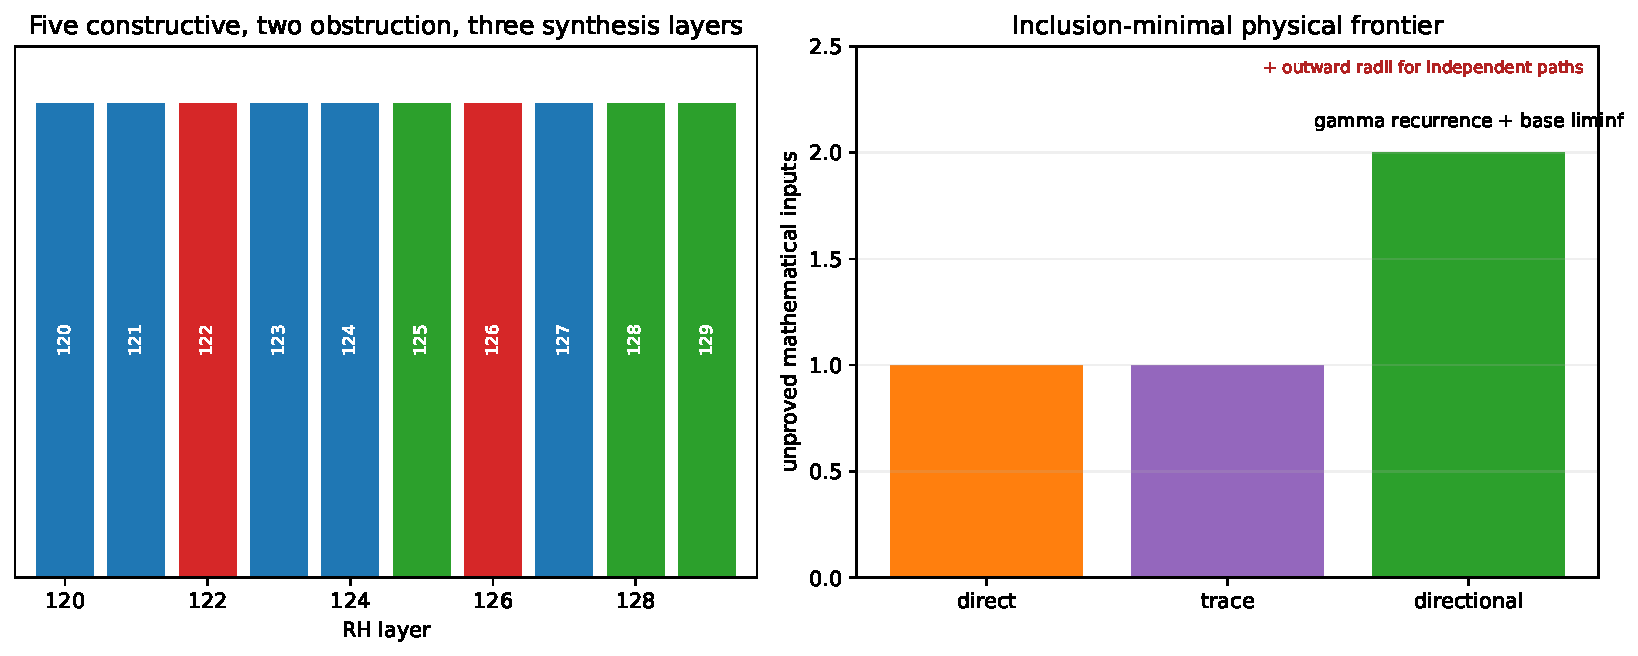
\includegraphics[width=\textwidth]{figures/ten_layer_gauge_recurrence_review.pdf}\caption{The ten-layer classification and the refined mathematical frontier.}\end{figure}

\section{Revised route}
The next finite gate should rebuild RH-121/RH-125 on one high-precision or
interval assembly, remove the positive Gram floor, work on the actual
supported subspace, and archive RH-127 radii.  If the directional advantage
survives, the theoretical priority is a natural gauge derived from the
memory and packet recursions, followed by source-level bounds on $\rho_n$,
$q_n$, and the normalized-base liminf.  The scalar direct and trace routes
remain on hold pending genuinely new source laws.

No all-level physical packet, uniform Stage A, Hilbert--Polya operator,
zeta-zero identification, or Riemann Hypothesis conclusion is claimed.
\bibliographystyle{plainnat}\bibliography{references}\end{document}
